\subsection{Improvements to the Slimpletic Integrator and their Physical Applications}
\label{sec:results-si}

\begin{figure}[t]
\label{fig:dho_energy_bounds}
  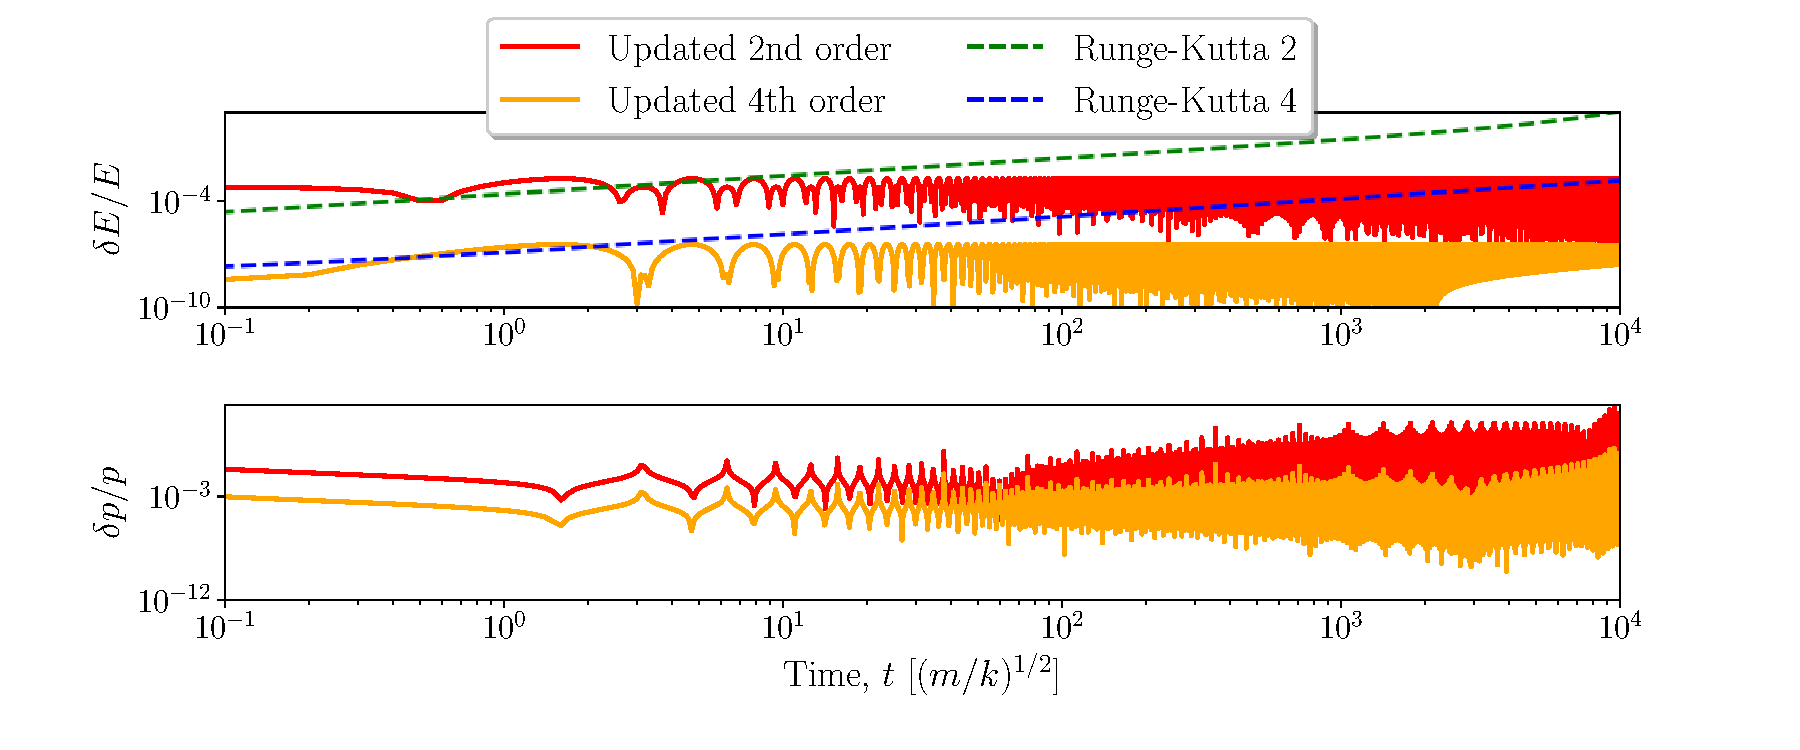
\includegraphics[width=\columnwidth]{figures/dho_energy_momenta_fractional_err.pdf}
  \caption{A comparison of the error in the energy, top, and momenta, bottom, as a fraction of the known analytic solution of the system, of the \updimpl{} simulating a damped harmonic oscillator. One can clearly observe that the fractional energy error is bounded and displays the oscillating behaviour that we expect from previous work, whereas the momenta error does not display such behaviour. This plot is based off its equivalent in the original paper \cite[Figure 2, bottom]{tsangSLIMPLECTICINTEGRATORSVARIATIONAL2015}.}
\end{figure}

As discussed we first verify that the required errors orders are preserved by the \updimpl{} when compared to the \orgimpl{} and traditional non-variational integrators. This can be seen in \fref{fig:dho_energy_bounds} where the fractional error of the system from the true analytic solution is compared directly against the performance of the \orgimpl{} and Runge-Kutta order 2 and 4. We clearly observe that the fractional energy error remains bounded across the timeframe of iteration. This is not the case for the fractional momenta error however as fixed-time-step variational methods such as those implemented cannot be both slimpletic-momentum and momentum-energy preserving \cite{zhongLiePoissonHamiltonJacobiTheory1988}.

\begin{figure}[t]
  \label{fig:dho-n-runtime}
  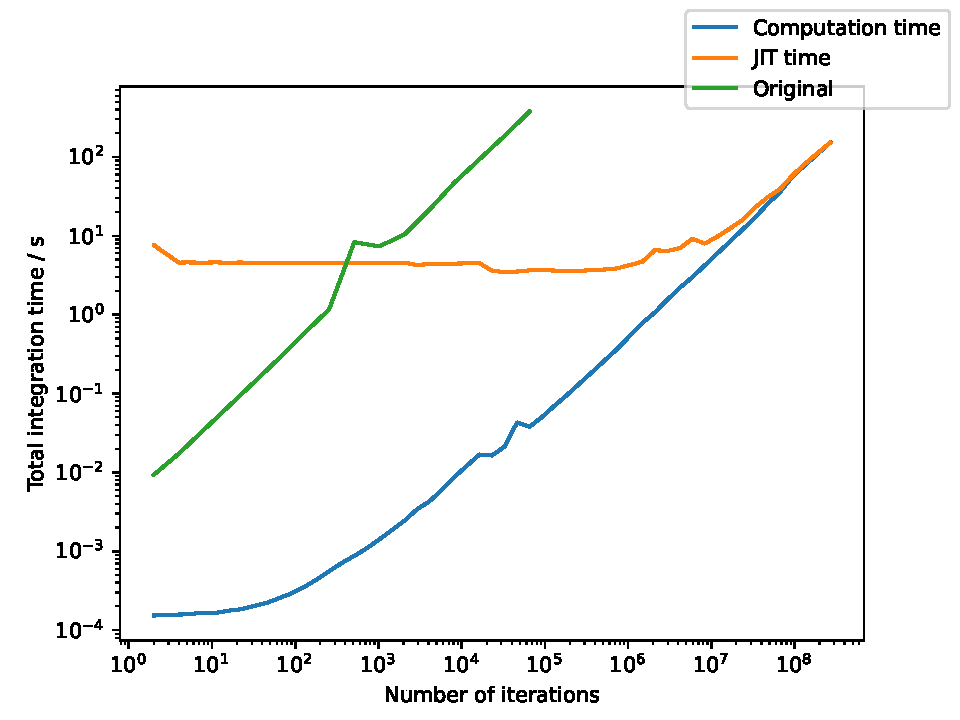
\includegraphics[width=\columnwidth]{figures/dho_n_runtime.pdf}
  \caption{A comparison of running a damped harmonic oscillator system for various numbers of iterations, with $r = 2, \Delta t = 0.1$. The \updimpl{} runtime is split into two components where \enquote{JIT time} represents the one time fixed cost of compiling the function (see \sref{sec:intro-autodiff}) and \enquote{Computation time} represents the actual time spent on computation.
  Each value is a mean of 4 runs, with the \orgimpl{} being cut off early due after $> 20$ minutes runtime for the next sample.}
\end{figure}

\begin{figure}[t]
  \label{fig:dho-r-runtime}
  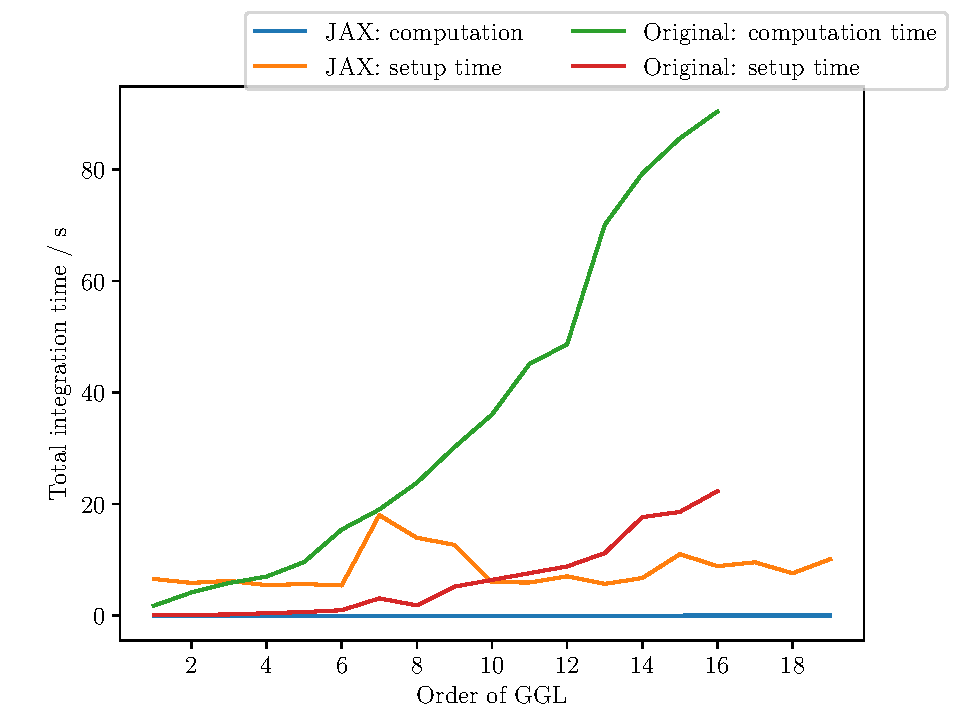
\includegraphics[width=\columnwidth]{figures/dho_r_runtime_linear.pdf}
  \caption{A comparison of running a damped harmonic oscillator system for various values of $r$, the order of the GGL quadrature, with $\Niter = 500, \Delta t = 0.1$. Each result being a mean of 4 independent runs.
	For both implementations we split the overall time into setup and computation as changing the method order requires re-discretising the Lagrangian and thus non-trivial work under both implementations.}
\end{figure}

Next we explored the time complexity of the system in terms of the iteration count, $N_{\text{iter}}$, and GGL quadrature order, $r$. These are important to physical applications as they determine the limits of iteration accuracy when iterating over large timescales, error scaling as $(\Delta t)^{2r + 2}$ and total timeframe being $N_{\text{iter}} \Delta t$.

Focusing first on the time complexity in $N_{\text{iter}}$ as shown in \fref{fig:dho-n-runtime}, we note that that the computation time of the \updimpl{} is much lower than that of the \orgimpl{}, with the \updimpl{} growing as $\Or(\Niter^a)$ where $a = 1.0140 \pm 0.0042$. In addition we note that the fixed cost JIT compilation remains roughly constant until growing linearly from about $10^7$ iterations.

This pattern is seen also in \fref{fig:dho-r-runtime} when investigating the time-complexity in the order of the method. Again the JIT time remains roughly constant across the domain tested, and though it starts out initially higher than than the \orgimpl{}'s setup costs, the \orgimpl{}'s computation time quickly swamps this fixed cost.
Similar to the behaviour in $\Niter$, the computation time for the \updimpl{} is also linear $r$ , remaining insignificant in the overall runtime. This is in comparison with the \orgimpl{} where the setup time grows as $\Or(r^n)$ with $n = {2.31 \pm 0.15}$ and the computation time as $\Or(r^m)$ with $m={1.490 \pm 0.070}$.

TODO: How do we report sig. fig again?

It should be noted that while increasing the order of the method will increase the precision, at higher orders we start encountering issues with the fixed precision \texttt{float64} type used for calculation in the \updimpl{} compared the the arbitrary precision numerics employed in the \orgimpl{}.
Still however this represents an overall improvement in accuracy in physically meaningful simulations as the required precision could be more readily attained by decreasing $\Delta t$ rather than increasing $r$, avoiding the blowup of runtime observed in the \orgimpl{}, or the degradation of precision at high $r$ in the \updimpl{}. 

TODO: This is where the lattice modelling will go.

%To end the direct application of the \updimpl{} to physical systems we exploit its ability to work on large collections of similar systems, across different choices of physical parameters and initial conditions without incurring the fixed costs discussed prior. To display this we choose to simulate a large collection of double pendulums, with damping on the fixed pendulum, from different initial conditions to observe the chaotic behaviour as seen in \fref{fig:ddp}.

%\begin{figure}[t]
%  \label{fig:ddp}
%  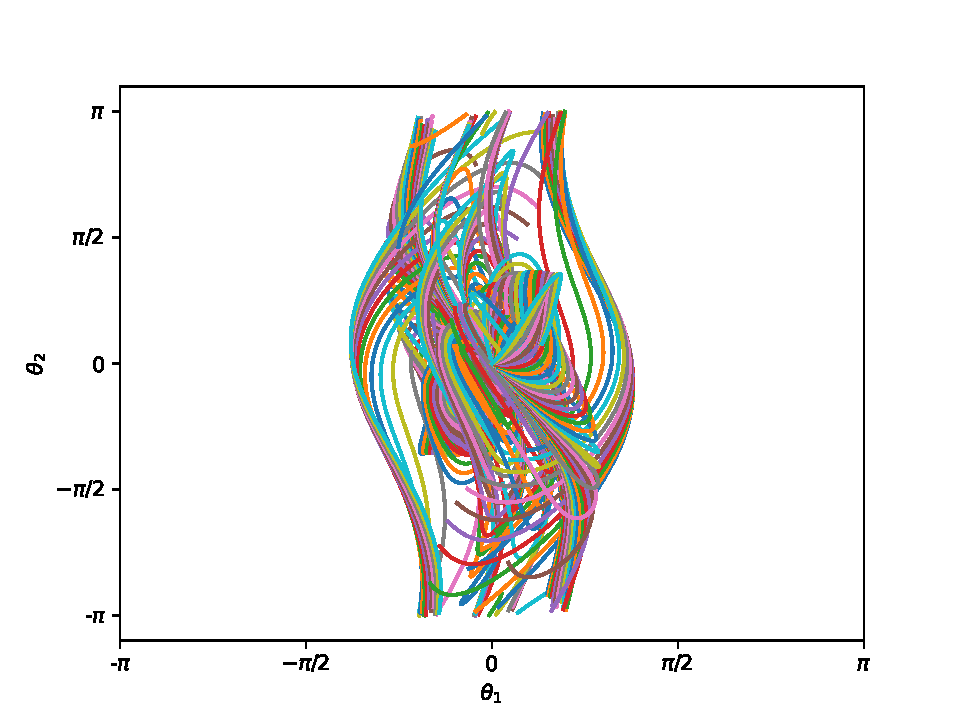
\includegraphics[width=\columnwidth]{figures/damped-double-pendulum.pdf}
%  \caption{Phase space plots of $\theta_1$ and $\theta_2$ for a double pendulum, pendulum 1 fixed, and pendulum 2 attached to 1. Both pendulums have uniform densities and unit mass and lengths. The fixed pendulum has damping applied which can be seen by the general spiral inwards over the duration of the lines. TODO: This isnt the cleanest but I want a physical simulation, can I do better?}
%\end{figure}

%\begin{enumerate}
%	\item Modelling of MD system
%	\item PRD? for physics?
%\end{enumerate}

% We got X% speed up
% TODO: This would be good to estimate. This means we can model Y% larger systems for Z% longer time frames

